\documentclass[11pt]{article} 
\usepackage{calc}
\usepackage{lettrine}
\usepackage[margin={1in,1in}]{geometry} 
\usepackage[hwkhandout]{hwk}
\usepackage[pdftitle={Mean Value Theorem},colorlinks=true,urlcolor=blue]{hyperref}
\usepackage{graphicx}
\usepackage{wrapfig}

\renewcommand{\theclass}{\textsc{math}1300: calculus I}
\renewcommand{\theauthor}{Tyson Gern}
\renewcommand{\theassignment}{Mean Value Theorem}
\renewcommand{\dateinfo}{section 3.10}
\renewcommand{\abstractname}{(BBC News)}

\newcommand{\ds}{\displaystyle}

\begin{document}
\drawtitle

\section*{Specs Spies on Speeding Motorists}

\begin{abstract}
  \noindent A new kind of speed trap is to be launched in a bid to cut
  deaths on one of Scotland's most dangerous roads.
\end{abstract}

\begin{wrapfigure}{r}{0.37\textwidth}
  \begin{center}
    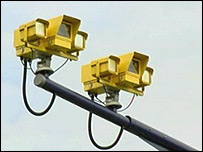
\includegraphics[width=0.3\textwidth]{camera.jpg}
  \end{center}
\end{wrapfigure}

\lettrine[lines=1]{T}{he Speed Enforcement Camera System} (Specs) will
track drivers over a 28-mile length of the A77 and calculate their
average speed.

The stretch of road between Ayr and Girvan is an accident blackspot
with 15 fatalities and 314 accidents between 1999 and 2004.

It was officially launched on Thursday with speeders facing various
penalties.

Those caught out by the Specs systems could end up having three points
added to their licence and a fine of at least \textsterling 60.

The \textsterling 775,000 initiative consists of 40 banks of hi-tech
cameras at points between Bogend Toll, north of Ayr, to Ardwell, south
of Girvan and is the largest in the UK.

The cameras are due to go live later in the month.

They have already been dubbed ``yellow vultures'' by drivers in England,
where they are currently operating, because of their colour and the
way they are perched on gantries above motorists.

Instead of taking the usual snapshot of a driver as they pass one
fixed point they measure the time it takes a vehicle to travel between
various points allowing the system to calculate its average speed.

\subsection*{Speed control}

The new system is the first major initiative to be implemented from a
wider \textsterling 20m programme of engineering improvements and
education initiatives, as well as a driver and community awareness
publicity campaign.

The Ayrshire pilot scheme will be assessed after a year and if
considered a success, it could be rolled out in other areas.

The project is being operated by the Strathclyde Speed Camera
Partnership, a joint initiative by police and local authorities.

Spokesman Neil Macgillivray said the aim was to encourage drivers to
slow down and thereby cut the number of accidents.

He said: ``The system will be launched with a great deal of publicity
and there will be advisory signs to remind drivers that they are in a
speed controlled zone.

``The primary aim of the safety cameras is to influence driver
behaviour and to improve safety along the route.

``Catching increased numbers of speeding motorists is not the aim.''

Justice Minister Cathy Jamieson officially unveiled the new cameras on
Thursday and said the Scottish Executive was ``determined'' to improve
safety along the A77.

\subsection*{`Overall strategy'}

Ms Jamieson said: ``I am convinced that the installation of Specs along
this route can play an important part in our overall strategy to
improve road safety on the A77 and will encourage better driving right
along the route.

``Let no one be in doubt - excessive speed is the cause of too many
injuries and deaths on our roads.''

Road safety campaign, the A77 Safety Group, welcomed the scheme and
thought it would improve conditions on the road.

The leader of South Ayrshire Council Andy Hill, which is part of the
group, said: ``The installation of this new camera system is, without
doubt, an important step forward in improving safety on the A77.

``Any initiative which can help to reduce the number of such accidents
is to be wholeheartedly welcomed.''

The AA also supported the measure but only as a temporary solution
until new and safer junctions are built.

However, some motoring groups claim it will not make any difference.

A spokesman for the Association of British Drivers said the cameras
could actually make the road less safe because drivers would
concentrate more on speed than what was happening on the road.

And the RAC questioned whether speed was the real problem.

Its head of traffic and road safety, Kevin Delaney, said: "We need to
look at the underlying causes of accidents and ask whether there could
be other factors, such as line of sight at junctions.

``If speed is not the main problem, then you end up with more cameras
generating more fines, more disgruntled motorists, but still the same
number of crashes.''

\vfill

\bibliographystyle{plain}
\nocite{*}
\bibliography{03.10refs}

\end{document}

%%%%%%%%%%%%%%%%%%%%%%%%%%%%%%%%%%%%%%%%%%%%%%%%%%%%%%%%%%%%%%%%%%%%%%
%%% Local Variables:
%%% mode: TeX-PDF
%%% End:
%%%%%%%%%%%%%%%%%%%%%%%%%%%%%%%%%%%%%%%%%%%%%%%%%%%%%%%%%%%%%%%%%%%%%%